\chapter{Summary, Discussion, \& Conclusion} \label{ch:conclusion}

\section{Chapter Purpose \& Structure}

This chapter has two purposes. The first is to review the previous chapters and summarize the contributions presented in each. This is the focus of Section \ref{sec:summary}. The second purpose is to supply an answer to Research Question 3:

\blockquote{What steps are necessary to establish \acf{evdt} as a continually development framework, a community of practice, and a growing code repository?}

This is the focus of Section \ref{sec:future-inquiry}, which accomplishes this by providing Research Deliverables 3a and 3b:
	\begin{enumerate}[label=\emph{\alph*},itemsep=0pt,parsep=0pt]
		\item{An assessment of lessons learned from these \acf{dss} development processes} 
		\item{An outline of potential future \ac{evdt} refinement and extension, such as using \ac{evdt} to inform the development of future \acf{eo} systems that are better designed for particular application contexts}
	\end{enumerate}
	
The chapter, and the thesis as whole, then ends with a brief concluding statement.

\section{Summary \& Contributions} \label{sec:summary}

\subsection{Theory \& Critical Analysis}

This thesis, due to its multidisciplinary aspect, did not have a singular literature survey, but instead had several distinct sections summarizing and analyzing existing literature. Chapter \ref{ch:theory} was the first of these. It discussed five distinct fields that are foundational to the \ac{evdt} Modeling Framework:

\begin{itemize}[itemsep=0pt,parsep=0pt]
	\item{\textbf{Section \ref{sec:sustainable_development} - Sustainable Development}. This term, which has grown enormously in popularity over the past couple of decades, encapsulates the desires to balance the sometimes aligning, sometimes conflicting needs for environmental protection, economic development, and advancement of human society (including health and wellness). The idea of such linkages between different domains, creating a complex system, underlies the \ac{evdt} framework.}
	\item{\textbf{Section \ref{sec:se} - Systems Engineering:} This discipline, which largely arose out of the need for a kind of meta-engineering for large aerospace projects, provides many of the tools and methods used by the \ac{evdt} Framework, including most notably the \acf{saf}.}
	\item{\textbf{Section \ref{sec:gis} - \acf{gis}:} This field provides the geospatial backbone to the analyses conducted and \acp{dss} created over the course of an \ac{evdt} project.} 
	\item{\textbf{Section \ref{sec:collaborative} - Collaborative Planning:} This field is where the \ac{evdt} Framework draws its means of engaging stakeholders to a greater extent that is common in systems engineering applications.}
	\item{\textbf{Section \ref{sec:dss} - \acf{dss}:} The goal of the \ac{evdt} Framework is to support sustainable development decision-making, so it is only natural that we draw upon the existing literature on methods of supporting decisions.}
\end{itemize}

Once summarized, these fields were then reconsidered through a critical lens in Section \ref{sec:critiques}. This was done to better understand the causes of various historical failings of each of these fields and how such pitfalls might be avoided when constructing and implementing a new framework. 

The first of these critiques focused on whether it is even possible to advance sustainable development, and its human wellness component in particular, through the use of technical means and expertise. This questions was considered both in the general case and as it applied to \ac{gis}, planning and international development, and systems engineering in particular. This analysis demonstrated that any given technology is not ethically neutral, but comes laden with intent, incentives, and constraints on its use; requiring us to be conscientious when designing new technologies. Specific steps to accomplish this include considering and involving a wide set of stakeholders during the design of a new system; focusing on supporting members of a community to make their own decisions, rather than prescribing a single ``optimal" decision from the outside; and maintain a certain level of epistemic humility about the capabilities of the technologies that we use.

The second critique considered whether sustainable development, as it is commonly defined and used, is actually an effective means of advancing environmental protection, social advancement, and economic development; or if its just a means of greenwashing the last of these. In particular it considered the utility of the \acfp{sdg}. In this analysis, I noted that there are several, legitimate critiques of the \acp{sdg}, including the perhaps over-focus on specific, quantifiable metrics, a largely top-down national perspective, and a lack of cross-goal connections. That said, I also noted several positive aspects of the \acp{sdg}, including their improvement upon the earlier \acfp{mdg} and their ability to facilitate communication about sustainable development. Ultimately, I conclude that the best approach for our new framework is to focus on more local, targeted, bottoms-up applications that have significant stakeholder involvement.

The third and final critique considered whether there is any evidence that \acp{dss}, and scenario planning in particular, have any demonstrable value. After discussing various cases of muddled evidence or even counterproductive results, I lay out the case for a participative, model-based form decision support that has firmer evidence and is reasonable grounds on which to base a doctoral dissertation.

Through the summaries and critiques, Chapter \ref{ch:theory} provided Research Deliverable 1a, ``A critical analysis of systems engineering, \ac{gis}, and the other fields relied upon in this work.", and one step towards answering Research Question 1:

\blockquote{What aspects of systems architecture (and systems engineering in general) can be used to support sustainability in complex \ac{sets}? In particular, how can they be adapted using techniques from collaborative planning theory and other critical approaches to avoid the technocratic excesses of the past?}

\subsection{The EVDT Framework}

Chapter \ref{ch:evdt} took these various foundational fields and lessons presented and used them to construct a methodology for constructing a \ac{dss} for sustainable development applications. It surveyed a variety of processes and projects that seek to accomplish similar goals. I found that there remained a need for a generalized framework that combined multidisciplinary model integration, stakeholder participation and collaboration on a local scale, and the significant use of remote observation data for sustainable development.

The remainder of the chapter was dedicated to walking through the new proposed process, entitled the \ac{evdt} Modeling Framework, shown in Figure \ref{fig:evdt_framework}, and constituted by five basic elements:

\begin{enumerate}[label=\emph{\Alph*)},itemsep=0pt,parsep=0pt]
	\item{The use of the \acf{saf} to understand the system context, identify stakeholder needs, and design the \ac{dss}.}
	\item{A conceptualization of the sustainable development application in terms of its Environment, Human Vulnerability and Societal Impact, Human Behavior and Decision-Making, and Technology Design components.}
	\item{An interactive \ac{dss}.}
	\item{A consideration towards modularity and re-use in future applications.}
	\item{Collaborative development of the \ac{dss} that continues beyond initial stakeholder engagement.}
\end{enumerate}

Through this guide, Chapter \ref{ch:evdt} provided Research Deliverable 1b: ``A proposed framework for applying systems engineering for sustainable development in an participatory and social-justice-oriented manner" and, together with the previous chapter, supplied an answer to Research Question 1. This chapter did not, however, provide any concrete demonstration or evaluation of the \ac{evdt} Modeling Framework. That was a task left to the following two chapters.

\subsection{Rio de Janeiro Development \& Mangroves}

The first of the two case studies, presented in Chapter \ref{ch:mangroves}, was on the development of a \ac{dss} for the setting of urban planning zones and environmentally protected areas in the western portion of the city of Rio de Janeiro, particularly around the Guaratiba area. It focused on the relationship between coastal mangroves and the local inhabitants, including the ecosystem services provided by the mangroves.

To accomplish this, I conducted a stakeholder analysis process via the \ac{saf}, coming to understanding the history of the Guaratiba area, its possible futures, and the relationships between many of its stakeholders. This process informed the design of a desktop-based \ac{dss} and the targets of a series of analyses that included tracking mangrove extent and health, estimating mangrove biomass and carbon sequestration, the value of various mangrove ecosystem services, and the impact of zoning and conservation policy on all of the above. The \ac{dss} compiled these in an interactive manner for use by stakeholders.

In doing so, I was able to supply the first instances of Research Deliverables 2a and 2b:

\begin{enumerate}[label=\emph{\alph*},itemsep=0pt,parsep=0pt]
	\item{System architecture analyses of each of the case studies.} 
	\item{Development of an \ac{evdt}-based \ac{dss} for each of the case studies.} 
\end{enumerate}

The onset of the \ac{covid} pandemic and the abrupt termination of the project resulted in an uncompleted Research Deliverable 2c, ``An interview-based assessment of the development process and usefulness of each \ac{dss}." Chapter \ref{ch:theory} was able to present both what feedback was received and the originally intended plan for collecting such feedback. Section \ref{sec:future-inquiry} below will also contain some additional evaluation of this case study.

\subsection{Vida DSS for COVID-19 Response}

The second of the two case studies, presented in Chapter \ref{ch:vida}, was on the development of two \acp{dss} for supporting \ac{covid} response policymaking in several different regions around the world, including Luanda, Rio de Janeiro, Regíon Metropolitana de Santiago, Java \& Sulawesi, Querétaro de Arteaga, and Boston. 

To pursue an \ac{evdt} project for so many study areas, a large team of Local Context Experts and Technical Area Experts (with some individuals serving in both capacities) was assembled. With their participation, we were able to conduct a wide variety of analyses, including on the impacts of \ac{covid} on air quality, nightlights, and human mobility. We also constructed two \acp{dss}, one desktop-based and one online, the former of which was capable of simulating \ac{covid} cases and other phenomena using a \acf{sir} model. 

This case study, in addition to the within-study-area stakeholder collaboration originally conceived by the \ac{evdt} Framework, had significant cross-study-area collaboration, providing additional benefits beyond the analyses and \acp{dss} that were the focus of this project. 

These actions were allowed to provide additional instances of Research Deliverables 2a, 2b, and 2c. As a result, we can now offer a tentative affirmative to Research Question 2:

\blockquote{Does the \ac{evdt} Modeling Framework effectively support decision-making in in complex \ac{sets}?}

\section{Lessons \& Opportunities for Future Inquiry} \label{sec:future-inquiry}

This section is dedicated to noting the certain limitations, lessons, and opportunities for future inquiry that have arisen out of the work presented in this thesis. In particular, it discusses each of these as they pertain to the \ac{evdt} Framework and the general methodology. For notes on limitations and opportunities connected to specific elements of analysis (such as air quality monitoring), refer to the Discussion section of the respective case study chapter.

I will first focus on each of the two case studies, recounting some of the lessons and opportunities noted in their respective chapters. Then I will take these and conduct a more wholistic evaluation of this thesis and the \ac{evdt} Framework in general.

Collectively, this section will supply both Research Deliverables 3a and 3b:

\begin{enumerate}[label=\emph{\alph*},itemsep=0pt,parsep=0pt]
	\item{An assessment of lessons learned from these \ac{dss} development processes.} 
	\item{An outline of potential future \ac{evdt} refinement and extension, such as using \ac{evdt} to inform the development of future \ac{eo} systems that are better designed for particular application contexts.} 
\end{enumerate}



%Chapter \ref{ch:conclusion} will review these lessons, including discussing how the case studies would have been performed differently in retrospect.

%The second portion of the chapter, Section \ref{sec:critiques}, turns towards to critiques of the literature and the concept of this thesis. It is an attempt to recognize and preemptively address potential pitfalls of the approach taken in this thesis. These are primarily fundamental or ethical concerns, as opposed to mere questions of implementation, the latter of which are largely held for Chapter \ref{ch:conclusion}.

\subsection{In Rio de Janeiro \& Mangroves Globally}

\textbf{The need for the two separate iterations of the \ac{saf}.} Earlier version of the \ac{evdt} Framework where not as strictly linear as Figure \ref{fig:evdt_framework}. Both the \ac{saf} and the \ac{evdt} components were viewed as spanning the entire project and not being particularly distinct, with only one iteration of the \ac{saf} explicitly called for. This led to ambiguity about whether the \ac{evdt} practitioner should be focusing the \ac{saf} process on the existing {sets} that the community is operating in or on the \ac{dss} that was to be developed. 

Through this case study and other projects, we realized that it is important to first use the \ac{saf} to define and provide information on the existing \ac{sets} that stakeholders live in, then frame that \ac{sets} using the \ac{evdt} components, and only then embark on the design of a \ac{dss} using the \ac{saf}. This helps to avoid putting the cart before the horse and forcing a particular pre-conceived solution architecture upon the stakeholders. 

\textbf{The importance of Local Context Experts.} While stakeholder participation and collaboration was key to the \ac{evdt} framework in even its earliest versions, the importance of Local Context Experts as discussed in Section \ref{sec:intended} was not fully appreciated. 

In particular the importance of having firm connections to multiple stakeholders can be critical to properly involving as many stakeholders as possible. Sometimes, however, such alignment with certain stakeholders is desirable even if it runs the risk of alienating others, but such a decision should be consciously and explicitly made. Ovienmhada et al., for example, working on environmental justice in carceral landscapes of the US, intentionally positioned the project as a social justice endeavor that was aligned with prison abolition activists \cite{ovienmhadaEnvironmentVulnerabilityDecisionTechnologyModelingFramework2021}. 

\textbf{The importance of appropriately scoping an \ac{evdt} project.} Involving as many stakeholders as possible and taking the multidisciplinary approach called for by the \ac{evdt} Framework can quickly cause a project to balloon out of the realm of feasibility. Care must be taken to ensure that the project remains within the resources of the direct participants, mediators, and developers.

\subsection{Lessons from COVID-19}

\textbf{The benefits of multi-study-area or multi-project communication and collaboration.} The Vida International Network has facilitated international collaboration, allowing participants to share innovations and insights from their \ac{covid} response efforts. It has also encouraged intra-country collaboration by providing a motivation for outreach between government officials, academic researchers, and community leaders in order to fill data gaps and answer pressing questions. This process has also raised awareness of the utility of space-based \ac{eo} data, potentially preparing participants for future pandemic and non-pandemic applications. 

The success of the multilateral Network meetings prompted us to continue such meetings for a more general EVDT community audience, as well as to consider other potential means of engagement such as webinars or online resources. This likely would not have occurred if we had continued to pursue more individual, siloed \ac{evdt} projects as was the norm.

\textbf{The importance of clearly scoped problem and use.} Overall, the Vida project included many unsuccessful experiments (such as monitoring vehicle traffic) and disconnected components (such as the separate in-situ and \ac{eo}-based air quality analyses). It resulted in some interesting results that did not find their way into the \ac{dss} proper or to supporting decision-making in other ways. This was partially due to the rushed stakeholder analysis, which was in turn due to the urgency of the situation and the complexity of multiple study areas. As such, it was potentially unavoidable in this case study but nonetheless represents a cautionary tale for future \ac{evdt} analyses.

\subsection{The Future of EVDT} \label{sec:future}

One final Research Question remains:

\blockquote{What steps are necessary to establish \ac{evdt} as a continually developing framework, a community of practice, and a growing code repository?}

This section will draw upon the lessons identified in the case studies to seek to answer this question. 

\textbf{Fulfill the potential of the Technology feedback loop in the \ac{evdt} formulation.} In Figure \ref{fig:model}, four equal components are shown: Environment, Vulnerability, Decision-making, and Technology. The last of these is part of a feedback loop connecting the models in a cycle. The case studies presented in this thesis did not full instantiate this and there is significant potential for future projects to do precisely that. 

For the Chapter \ref{ch:mangroves} case study, there is the potential to extend the \ac{dss} and analyses to support the selection of \ac{eo} data sources that would better support the needs of the Guaratiba area. In Chapter \ref{ch:vida} case study, there is the possibility of providing support to decision-makers regarding the \ac{covid} testing regime. Future projects could involve using tradespace exploration or other tools to support the design of a new \ac{eo} satellite to meet the needs of some set of stakeholders.  

One proposed conceptualization of the \ac{eo} application value chain has the eight steps shown in Figure \ref{fig:eochain}  \cite{hakimdavarTransboundaryWaterImproving2018, woodPartnershipsEnableEarth2017}. Space agencies frequently find themselves not only providing steps 1-3 (their specialty) but also some combination of 4-8. The \ac{evdt} projects presented in this thesis primarily focus on steps 4-8. A fully fleshed out Technology component and feedback loop, however, has the potential to ``close the loop," connecting step 8 back to step 1. This would result in \ac{eo} systems more closely tied to the application needs of particular stakeholders and thus in better decision support. Such projects are already being pursued by other members of the Space Enabled research group, including on supporting the design of an Italian \ac{eo} system and for space sustainability decision support.

\begin{figure}[ht]
    \centering
    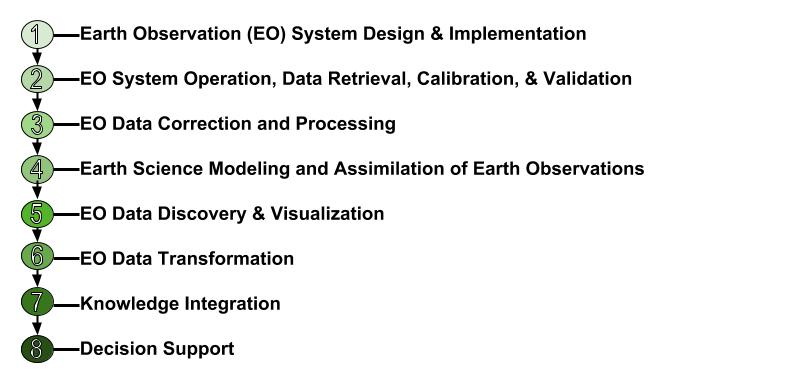
\includegraphics[width=0.7\textwidth]{Figures/chap7/EOChain.jpg}
    \caption{Generic Earth Observation Data Value Chain}
    \label{fig:eochain}
\end{figure}

\textbf{Conduct rapid prototyping \& co-design, without sacrificing stakeholder analysis.} In order to confirm that the proper data and dynamics are being captured, as well as to ensure the utility of the model to decision-makers and designers, the key stakeholders must be involved at all stages of the design process. Additionally, since most individuals have a difficult time providing concrete advice and criticism when discussing the abstract, rapid prototyping and mock-ups are important for stimulating feedback. One key component of this is always making sure that the user interface is available in the native language of the primary users.

Pursuing such rapid prototyping should not be allowed to cause the initial iteration of the \ac{saf} or the stakeholder analysis portion in particular to be sacrificed. The Chapter \ref{ch:vida} did precisely this, resulting in a series of analyses and \ac{dss} components that were not as well connected to each other and to stakeholder needs as should have been the case.

\textbf{Enlist appropriate experts and stakeholders.} The design of any \ac{eo} system is inherently interdisciplinary and this is also true for \ac{eo} applications. For this reason the development necessarily involves a wide range of collaborators who vary both in terms of discipline (systems engineering, urban planning, earth science, economics, etc.) and it terms of institution (academic researchers, government officials, \ac{ngo} and corporate leaders, local activists, etc.). Rather than make assumptions when confronted with an issue outside our expertise, we must our utmost to recruit or consult with a relevant expert. 

A key part of this is recognizing that these experts and stakeholders will have their own perspectives and priorities that will not always align. This is one of the primary purposes of the \ac{saf}: to understand and synthesize these perspectives. But it is also important to recognize that, particularly if the \ac{evdt} moderator is outside of the target community, one must be intentional with how one aligns (or appears to align) with the various stakeholders. Finding a relatively neutral actor to serve as a primary Local Context Expert can be quite useful for enabling productive collaboration with a wide range of stakeholders, as can independently cultivating relationships with different stakeholders. This was done in the Chapter \ref{ch:mangroves} case study, for example. Other projects however call for a more clear declaration of one's stance, even if this risks alienating certain stakeholders.

\textbf{Maintain open access and modularity for adaptation and reuse, without overly sacrificing usability.} The intent is not for the \ac{evdt} Framework is not to develop complete, black-box products, but rather to facilitate the development of widely accessible \acp{dss}. Part of this includes the collaborative aspect of the \ac{evdt} Framework, but another part is making the code itself readily available online and designing the analyses and \ac{dss} to be as reusable as possible. This helps prevent the monopolization of information that characterized some of the technocratic excesses discussed in Chapter \ref{ch:theory}. It also helps to ensure that new \ac{evdt} projects may, for example, be able to reuse previous \ac{eo} data processing techniques, while focusing on the vulnerability or decision-making components.

At the same time, a rigid fixation on maximal open access and reusability should not be allowed to significantly detract from usability. The case studies from Chapters \ref{ch:mangroves} and \ref{ch:vida} perhaps ran amiss here, focusing too heavily on custom, open source, desktop-based \acp{dss} that limited there ability to be easily accessed and used by stakeholders with a wide range of technical competence. This can be contrasted with Jaffe's online \ac{dss}, which saw wider use \cite{jaffeEnvironmentalEconomicSystems2022}. Such cloud-based and internet-hosted tools can eliminate the need to direct possession of high performance computing equipment by either the end users or the developers. This reduces cost-of-entry for potential developers of \ac{evdt} models and ensures that end users can interact with, critique, and apply the models wherever they are, provided they have internet access. In general, implementers of future \ac{evdt} projects should, during the \ac{saf} process, be particularly attentive to existing decision-making processes of different stakeholders and design the \ac{dss} to fit well within them.

\textbf{Seek to build relationships and collaboration across \ac{evdt} projects.} One of the key findings of the Vida case study in Chapter \ref{ch:vida} was that there is significant utility in providing venues for communication and collaboration across study areas or even across \ac{evdt} projects. Some of these benefits are to the \ac{evdt} projects themselves, identifying potential new topics of analysis or providing opportunities for the re-use of code and other assets across projects. Some of these benefits are outside of the \ac{evdt} projects themselves but still quite useful in their own right. These can include peer-to-peer learning and instruction on other sustainable development topics.
 

\section{Advancing Stakeholder-Informed Sustainable Development Decision-making}

This dissertation presented a new framework for supporting sustainable development decision-making. The goal of the research was to demonstrate both the need for and the usefulness of this framework, and to thereby advance sustainable development action, particularly on the local scale. To address these goals, I undertook three main research efforts. First, I conducted a critical analysis of a variety of fields relevant to sustainable development (including the concept of sustainable development itself) to identify potential points of synergy and how to avoid historical pitfalls. Second, I built upon this analysis to develop the \acf{evdt} Framework. Third, I demonstrated the framework in two case studies, one a rather straightforward application and one a significant deviation that still contained useful lessons. In pursuing these case studies, I also provided useful analyses and tools to stakeholders.

As might be expected for a project of this scope, I did encounter various challenges. Some of these challenges were internal to each case study and involved such things as the availability of data and understanding of the dynamics of the underlying phenomena. Some were part of the implementation, including a failure to conduct detailed usability studies or an urgency-and-complexity-based divergence from the \ac{evdt} Framework. Both provided useful lessons and the opportunity for future work.

It is my hope that the work presented in this thesis, I helped to fulfill a need for a generalized framework that combined multidisciplinary model integration, stakeholder participation and collaboration on a local scale, and the significant use of remote observation data for sustainable development. More broadly, I hope that this project serves to bridge the gap between disciplines (such as systems engineering and urban planning) and between stakeholders (such as academics, government officials, and members of the public) as we jointly try to pursue a more just and sustainable world.


